\documentclass[12pt]{article}
\usepackage[margin=2.5cm]{geometry}
\usepackage{enumerate}
\usepackage{amsfonts}
\usepackage{amsmath}
\usepackage{fancyhdr}
\usepackage{amsmath}
\usepackage{amssymb}
\usepackage{amsthm}
\usepackage{mdframed}
\usepackage{graphicx}
\usepackage{subcaption}
\usepackage{adjustbox}
\usepackage{listings}
\usepackage{xcolor}
\usepackage{booktabs}
\usepackage[utf]{kotex}
\usepackage{hyperref}

\definecolor{codegreen}{rgb}{0,0.6,0}
\definecolor{codegray}{rgb}{0.5,0.5,0.5}
\definecolor{codepurple}{rgb}{0.58,0,0.82}
\definecolor{backcolour}{rgb}{0.95,0.95,0.92}

\lstdefinestyle{mystyle}{
    backgroundcolor=\color{backcolour},
    commentstyle=\color{codegreen},
    keywordstyle=\color{magenta},
    numberstyle=\tiny\color{codegray},
    stringstyle=\color{codepurple},
    basicstyle=\ttfamily\footnotesize,
    breakatwhitespace=false,
    breaklines=true,
    captionpos=b,
    keepspaces=true,
    numbers=left,
    numbersep=5pt,
    showspaces=false,
    showstringspaces=false,
    showtabs=false,
    tabsize=1
}

\lstset{style=mystyle}

\pagestyle{fancy}
\renewcommand{\headrulewidth}{0.4pt}
\lhead{Hyungmo Gu}
\rhead{CSC369 Week 1 Notes}

\begin{document}
\title{CSC369 Week 1 Notes}
\author{Hyungmo Gu}
\maketitle

\section{Intro to OS}

\bigskip

\begin{itemize}
    \item What is Operating System
    \begin{itemize}
        \item is the program that manages the computer hardware
        \item is the software layer between user applications and hardware
        \item is used for
        \begin{itemize}
            \item Allication of resources
            \item Management of memory, security, etc.
        \end{itemize}

        \begin{center}
        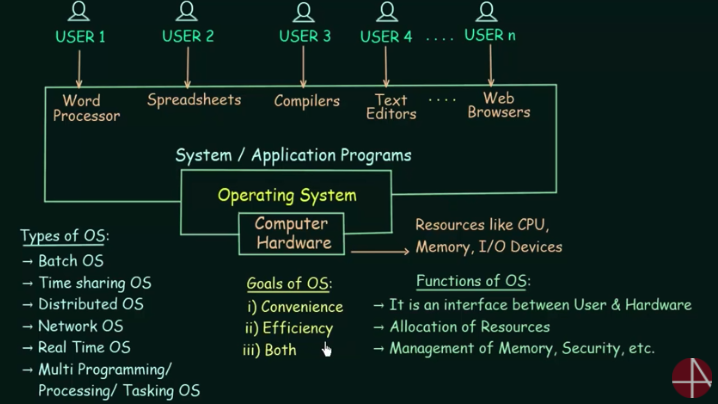
\includegraphics[width=\linewidth]{images/week_1_notes_1_1.png}
        \end{center}
    \end{itemize}
    \item Overview of Computer System

    \bigskip

    \begin{center}
    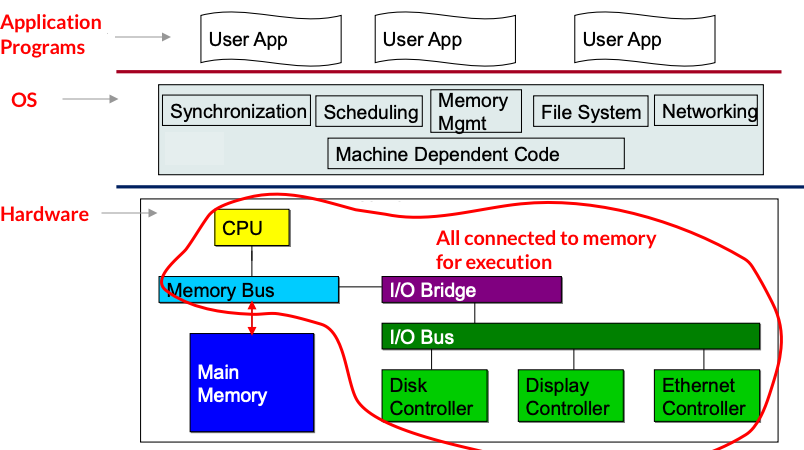
\includegraphics[width=\linewidth]{images/week_1_notes_1_2.png}
    \end{center}

    \bigskip

    \begin{itemize}
        \item All hardware devices are connected through common \textbf{bus} and are
        loaded to memory for execution.
        \item \textbf{Synchronization:} to ensure orderly acces to the shared memory
    \end{itemize}

    \item Storge Hierarchy / Storage Structure

    \bigskip

    \begin{center}
    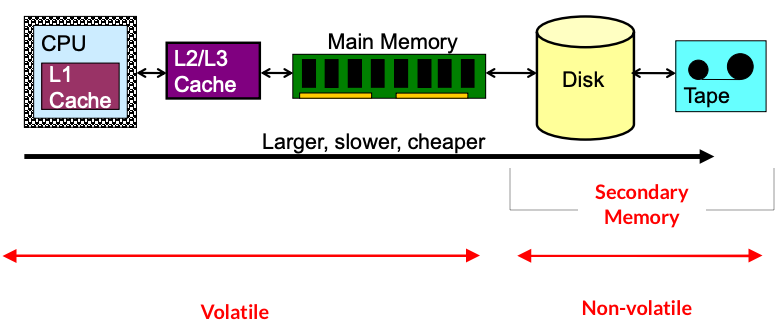
\includegraphics[width=\linewidth]{images/week_1_notes_1_3.png}
    \end{center}

    \begin{itemize}
        \item \textbf{Volatile $\to$} Loses contents when power is removed
        \item \textbf{Non-volatile $\to$} Retains contents even when power is removed
    \end{itemize}

    \item Caching / Cache Memory

    \begin{itemize}
        \item Is also called \textbf{Static Random Access Memory (SRAM)}
        \item Is more costly
        \item Hides performance differences when large access-time gap exsists
        between two levels
        \begin{itemize}
            \item Quad-quare requesting RAM for information

            \begin{center}
            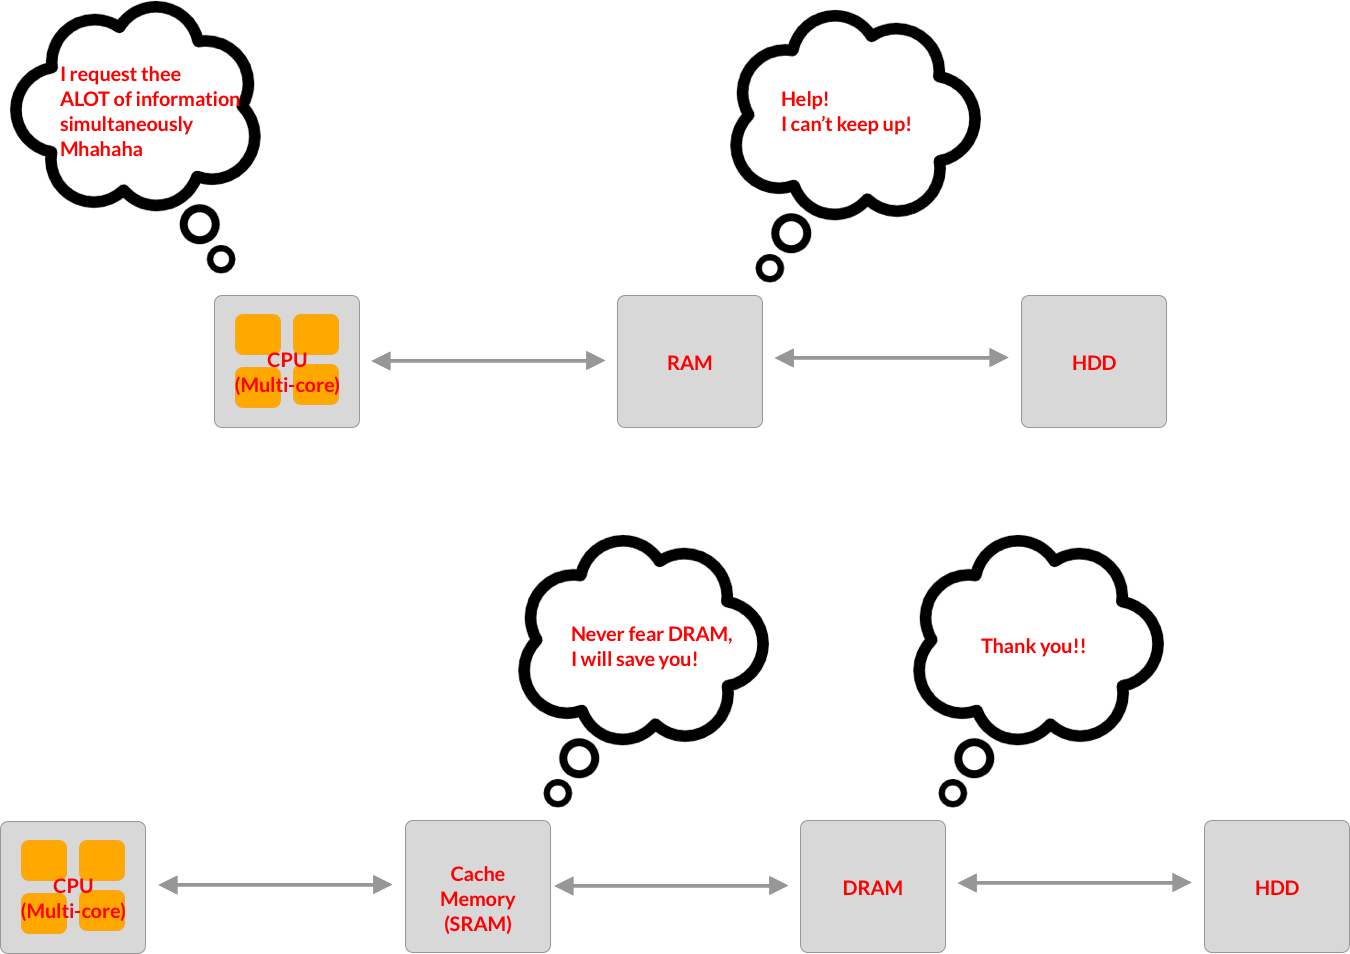
\includegraphics[width=\linewidth]{images/week_1_notes_1_4.png}
            \end{center}

        \end{itemize}
        \item More can be found \href{https://www.youtube.com/watch?v=Zr8WKIOIKsk}{here}
    \end{itemize}
    \item Concurrency
    \begin{itemize}
        \item Is execution of several instruction sequences at same time
        \begin{itemize}
            \item i.e, CPU and device controllers
        \end{itemize}
        \item \textbf{Interrupt:} are signals sent to the CPU by external devices,
        (usually I/O devices)
        \begin{itemize}
            \item It's like telling `Hey CPU, please stop this process, and do $y$
            instead, since this is more important'
            \item i.e. Network Packet has arrived, Disk I/O comeplete
            occured
        \end{itemize}
        \item \textbf{System Call:} are interrupt signals sent by software
        \begin{itemize}
            \item Is a programmatic way of a program requesting for service to
            kernel of operating system
            \item i.e. Accessing a hard-disk drive
        \end{itemize}
        \item IMPORTANT: An operating system is an \underline{event-driven} program.
    \end{itemize}
\end{itemize}

\bigskip

\section{Process Threads}

\bigskip

\begin{itemize}
    \item Part 1: The Process Concept
    \begin{itemize}
        \item \textbf{Process:} is a program in execution
        \item \textbf{Threads:} is the unit of execution within a process.

        \begin{align}
            \text{Thread} = \frac{\text{Job}}{\text{Unit of Work}}
        \end{align}

        \begin{itemize}
            \item A process can have anywhere from one thread to many threads
        \end{itemize}
    \end{itemize}

    \item Process Data Structure (PCB)
    \begin{itemize}
        \item Is called Process Control Block
        \item Is OS data structur representing each process
        \item Generally includes
        \begin{enumerate}
            \item Process State
            \begin{itemize}
                \item(Ready, running, blocked)
            \end{itemize}
            \item Program Counter
            \begin{itemize}
                \item Is an address that indicates the line of code
                that has to be executed next
                \item i.e. the next line of code i need to execute is line 2 :)

\begin{lstlisting}[language=c]
print("Hello World");
print("Hi World!") //<- Line 2
\end{lstlisting}

            \end{itemize}
            \item CPU Register \textit{**Need to come back}
            \item CPU Scheduling Information
            \begin{itemize}
                \item Priority of process
                \item Higher the priority $\to$ executed first
            \end{itemize}
            \item Memory Management \textit{**Need to come back}
            \item I/O Status Information
            \begin{itemize}
                \item Is list of input output devices assigned to this process
                \item Is used during execution
                \item i.e. Sound, Mouse, Keyboard
            \end{itemize}
        \end{enumerate}
    \end{itemize}

    \item Process States \& State Changes

    \begin{center}
    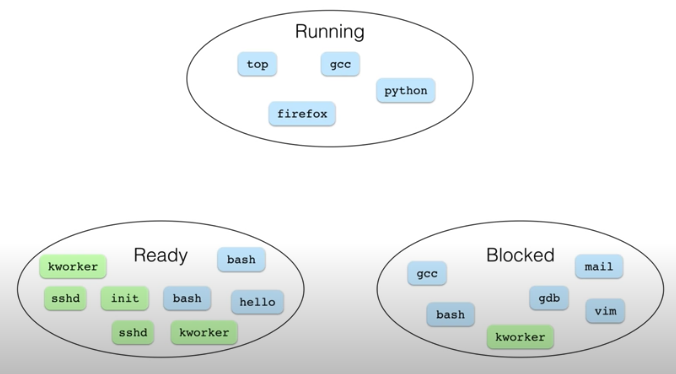
\includegraphics[width=0.8\linewidth]{images/week_1_notes_1_5.png}
    \end{center}

    \item State Queues

    \begin{itemize}
        \item Is a part of \textbf{process scheduling}
        \begin{itemize}
            \item keeps CPU busy at all times to deliver minimum response time
            for all programs

            \begin{center}
            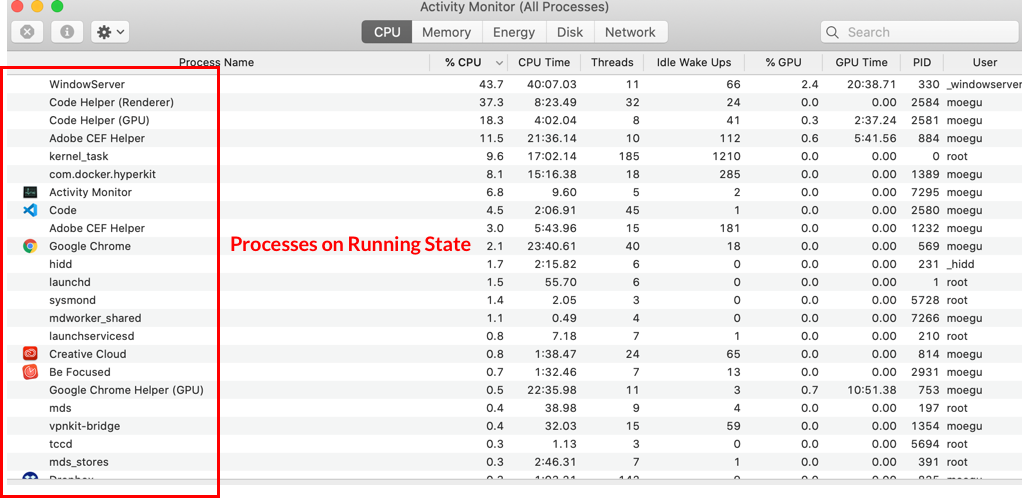
\includegraphics[width=\linewidth]{images/week_1_notes_1_6.png}
            \end{center}

            \item Here, processes in queue are \underline{switched} so frequently that
            user can interact with each program while running

        \end{itemize}
        \item Has one state queue for each process state
        \begin{itemize}
            \item Job Queue, Ready Queue, Waiting Queue, Blocking Queue
        \end{itemize}

        \begin{center}
        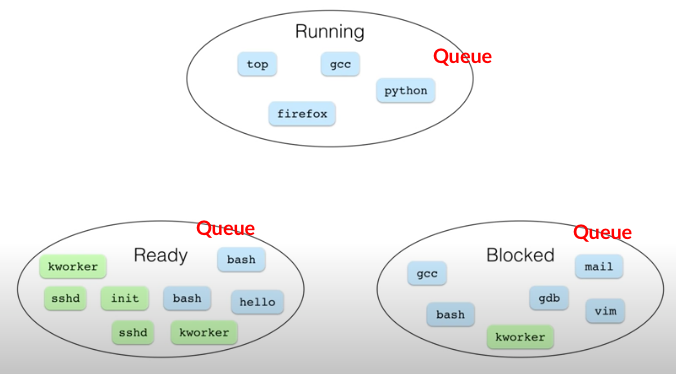
\includegraphics[width=\linewidth]{images/week_1_notes_1_7.png}
        \end{center}
    \end{itemize}

    \item PCBs And State Queues
    \item Context Switch
    \item Operations on Processes
    \item Process Creation
    \item fork()
    \item Duplicating Address Processes
    \item Divergence
    \item
\end{itemize}

\end{document}